\chapter{Resultados}

Con el fin de determinar si los modelos de estrellas de neutrones obtenidos con las ecuaciones de estado de la materia densa disponibles en la literatura son físicamente viables, se resolvieron las ecuaciones de TOV \eqref{dmtov},\eqref{dptov} y \eqref{dnutov} para un amplio rango de densidades centrales y se evaluaron las condiciones C1-C11 presentadas en la Sección \ref{phyacep}.

En la siguiente sección se describirá el proceso de verificación detalladamente para la EOS ENG \cite{Engvik1994}, dado que predice una masa máxima $M_{\text{TOV}}$ superior a la masa del pulsar MSP J0740+6620 \cite{Cromartie2019} y además satisface los límites más conservadores impuestos por la primera observación de ondas gravitacionales por la fusión de dos estrellas de neutrones GW170817 y su contraparte electromagnética \cite{Rezzolla2017,Radice2018,Ruiz2018,Shibata2019}. Después se presentarán los resultados consolidados para un conjunto representativo de 37 EOSs (incluyendo ENG) basados en la elección de EOSs presente en la revisión \cite{Ozel2016}.

\section{Un caso particular: la ecuación de estado ENG}

ENG es una EOS para materia compuesta de neutrones, protones, electrones y muones asimétrica (con fracciones de protones distintas a $1/2$) que usa un enfoque miscroscópico (de acuerdo a la clasificación presentada en la Sección \ref{EOS}) basada en el método de Dirac-Brueckener-Hartree-Fock. 

Los requisitos mínimos de consistencia física que una ecuación de estado debe cumplir son la condición de energía dominante (C6) y la condición de causalidad (C7). Estas condiciones dependen enteramente de la construcción de la ecuación de estado y pueden ser verificadas sin necesidad de resolver las ecuaciones de TOV. En las Figuras \ref{DECeng} y \ref{SSCeng} se verificó que la EOS ENG cumple las condiciones C6 y C7.

\begin{figure}[H]
   \begin{minipage}[b]{.48\textwidth}
        \centering
        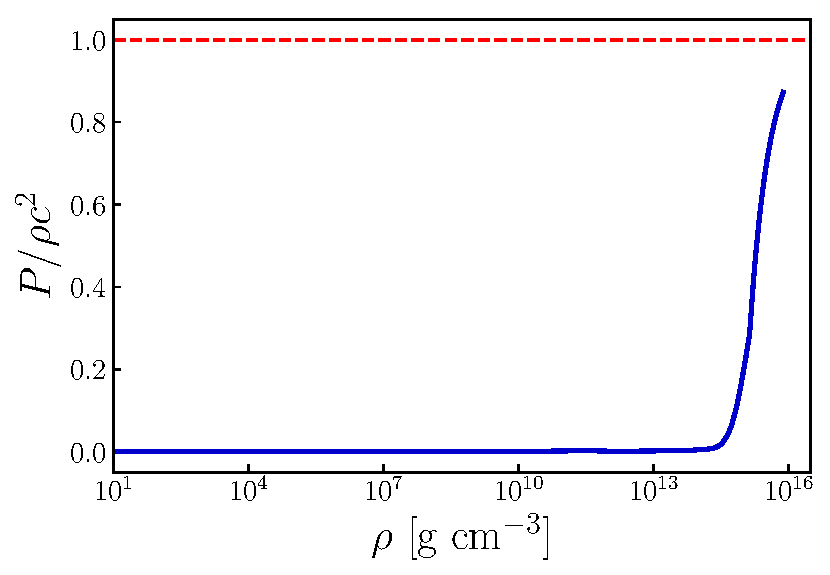
\includegraphics[width=1\textwidth]{figures/ECeng.pdf}
        \caption{Verificación de C6 para la EOS ENG. La línea roja punteada indica la igualdad $P=\rho c^2$. Se aprecia que $P/\rho c^2 \leq 1$, por lo que esta ecuación de estado cumple C6.}
        \label{DECeng}
    \end{minipage}
    \quad
    \begin{minipage}[b]{.48\textwidth}
        \centering
        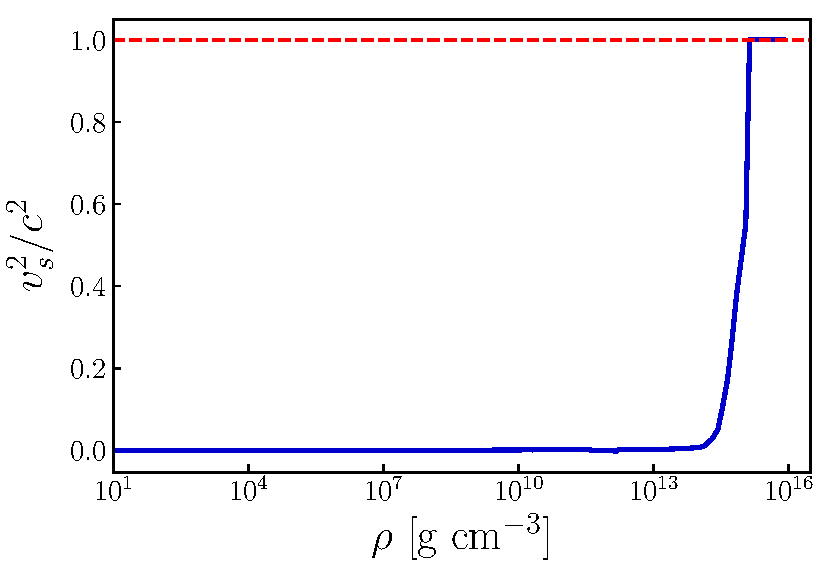
\includegraphics[width=1\textwidth]{figures/SSeng.pdf}
        \caption{Verificación de C7 para la EOS ENG. La línea roja punteada representa $v_s=c$. Se aprecia que $v_s^2/c^2 \leq 1$, por lo que esta ecuación de estado cumple C7.}
        \label{SSCeng}
    \end{minipage}
\end{figure}



\begin{figure}[H]
    \centering
    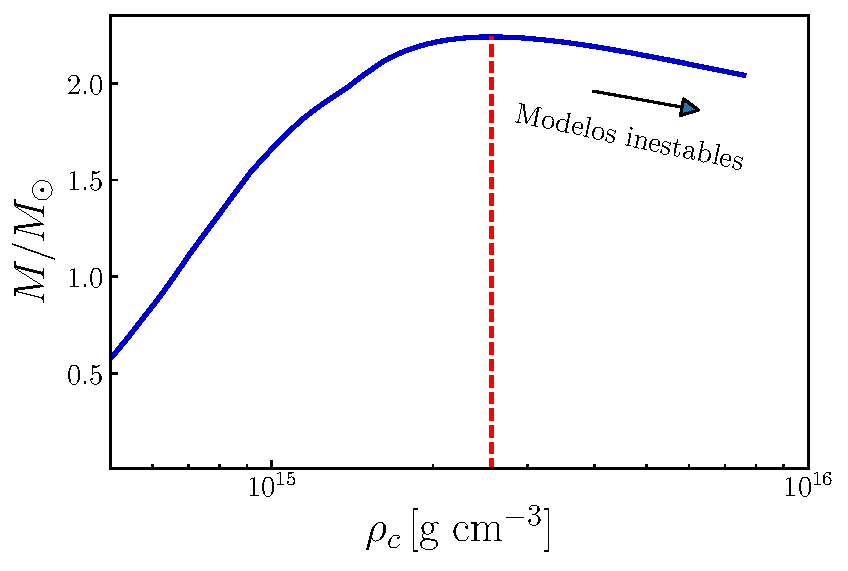
\includegraphics[width=0.7\linewidth]{figures/Mrhorel_eng.pdf}
    \caption{Identificando los modelos que no satisfacen C10. La masa máxima para esta ecuación de estado fue $M_{max}=2.241\,M_{\odot}$ alcanzada con la densidad central $\rho_c=2.5704 \times 10^{15}$ (línea roja punteada), así que modelos con $\rho_c \geq 2.5704 \times 10^{15}$ serán inestables ante pulsaciones radiales. }
    \label{mrhoeng}
\end{figure}

Tras confirmar que la ecuación de estado cumple C6 y C7, se procede a solucionar las ecuaciones de TOV para un conjunto de densidades centrales (valores iniciales) que típicamente va desde $\rho_c=\rho_0 \sim 10^{14} \text{g cm}^{-3}$ hasta la máxima densidad disponible en la ecuación de estado. Como las soluciones cumplen las condiciones de acoplamiento (C2) por construcción (como es descrito en el Apéndice \ref{NumSol}), se usa la condición C10 para restringir los modelos a analizar: sólo se considerarán modelos con densidades centrales tales que $\frac { \partial M \left( \rho _ { c } \right) } { \partial \rho _ { c } } > 0$. Esta derivada es nula para la configuración con masa máxima y se presenta un cambio del signo de la derivada de positiva a negativa, la densidad central para la que esto ocurre indica el inicio de las configuraciones inestables (ver Figura \ref{mrhoeng}).

Para continuar con el análisis de la estabilidad de los modelos que satisfacen C10 se halló la primera y segunda derivada respecto a la coordenada radial $r$ de $\rho$ y $P$ numéricamente (los detalles de cómo se obtuvo las derivadas numéricamente se encuentran en la Sección \ref{NumDer} del Apéndice \ref{NumSol}) con el objetivo de verificar las condiciones C9 y C11.  

Haciendo un análisis gráfico de $\dv{P(r)}{r} $ (ver Figura \ref{CrackStabilityeng}) se determinó que todos los modelos que satisfacen C10 también satisfacen C9. 
 

\begin{figure}[H]
    \centering
    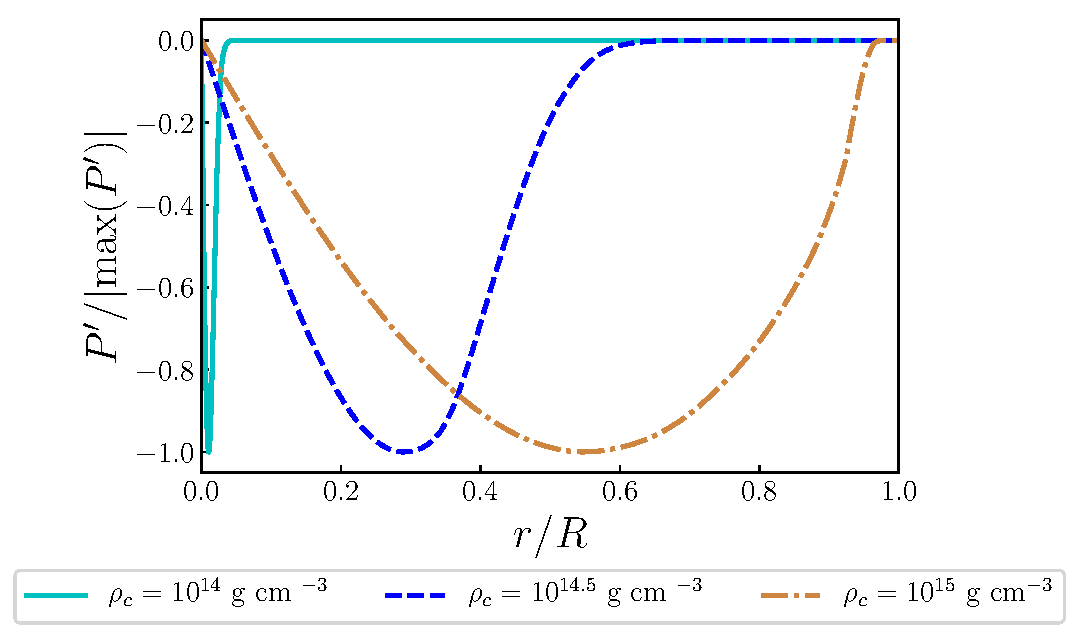
\includegraphics[width=0.93\linewidth]{figures/CrackStabilityeng.pdf}
    \caption{Verificación de C9. Se presentan los gradientes de presión de una muestra representativa de los modelos que cumplen con C10. Estos siempre son menores  iguales a cero  y por lo tanto los modelos considerados son estables ante cracking.}
    \label{CrackStabilityeng}
\end{figure}

Por otro lado, el análisis gráfico de $\dv[2]{\rho}{r}$ reveló que en todos los modelos hay una región en la cual no se cumple la condición C11 (ver Figura \ref{ConvecStabilityeng}). Al graficar $\dv[2]{\rho}{r}$ contra $\rho$ (ver Figura \ref{ConvecStabilityengCorrel}) se identifica que la zona que no cumple la condición C11 está acotada entre densidades cercanas a $\rho_{ND}\approx 4 \times 10^{11} $ y densidades cercanas $\rho_0$ (aŕea sombreada). Este rango de densidades concuerda con las encontradas en la corteza interior (ver Figura \ref{NSS}) y sugiere que la corteza interior hace que los modelos obtenidos con la EOS ENG sean inestables antes ante convección adiabática. 

\begin{figure}[H]
    \centering
    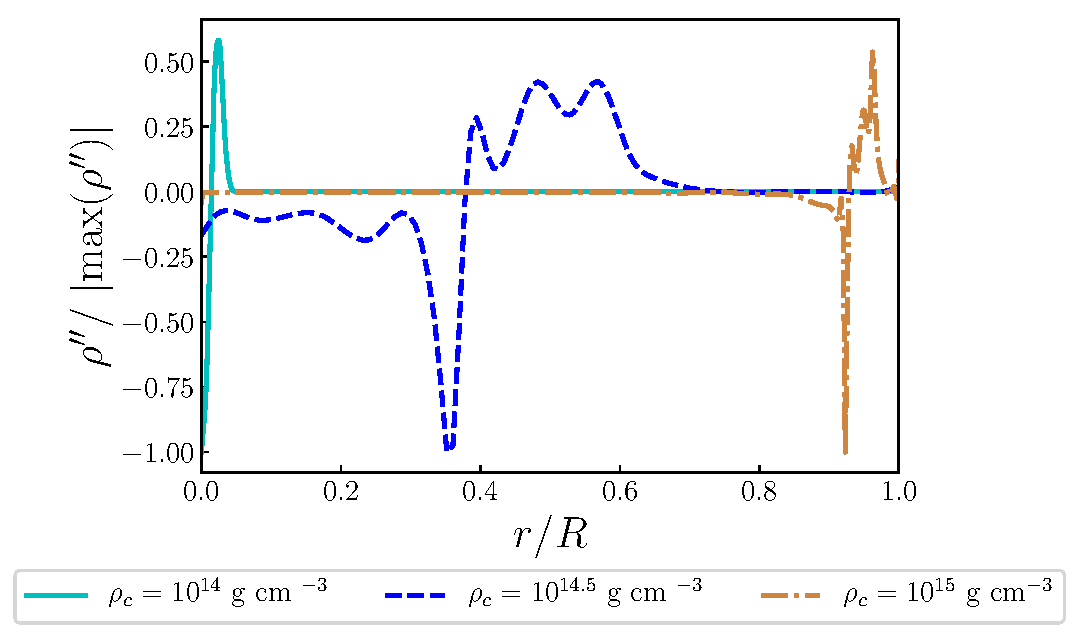
\includegraphics[width=0.93\linewidth]{figures/ConvecStabilityeng.pdf}
    \caption{Verificación de C11. Se presenta $\rho^{\prime\prime}(r)$ de una muestra representativa de los modelos que cumplen con C10. La condición no se cumple en toda la estrella para todos los modelos. }
    \label{ConvecStabilityeng}
\end{figure}
\begin{figure}[H]
    \centering
    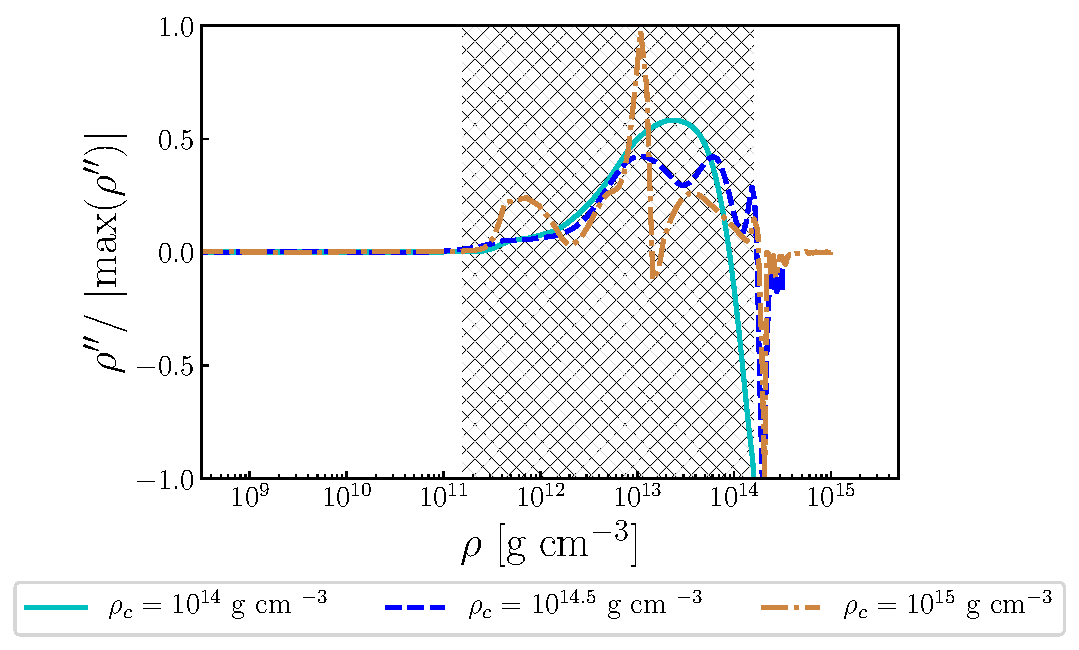
\includegraphics[width=0.93\linewidth]{figures/ConvecStabilityengCorrel.pdf}
    \caption{El gráfico $\rho^{\prime\prime}(\rho)$ permite identificar la ubicación de las inestabilidades: para todos los modelos se encuentran en el rango de densidades ($\rho_{ND},\rho_0$), lo que indica que se trata de la corteza interior de la estrella.} 
    \label{ConvecStabilityengCorrel}
\end{figure}

Finalmente se verificó que los modelos considerados son consistentes con la condición C3 calculando el corrimiento al rojo como función de la coordenada radial \eqref{redshift} (ver Figura \ref{Redshifteng}). 

\begin{figure}[H]
    \centering
    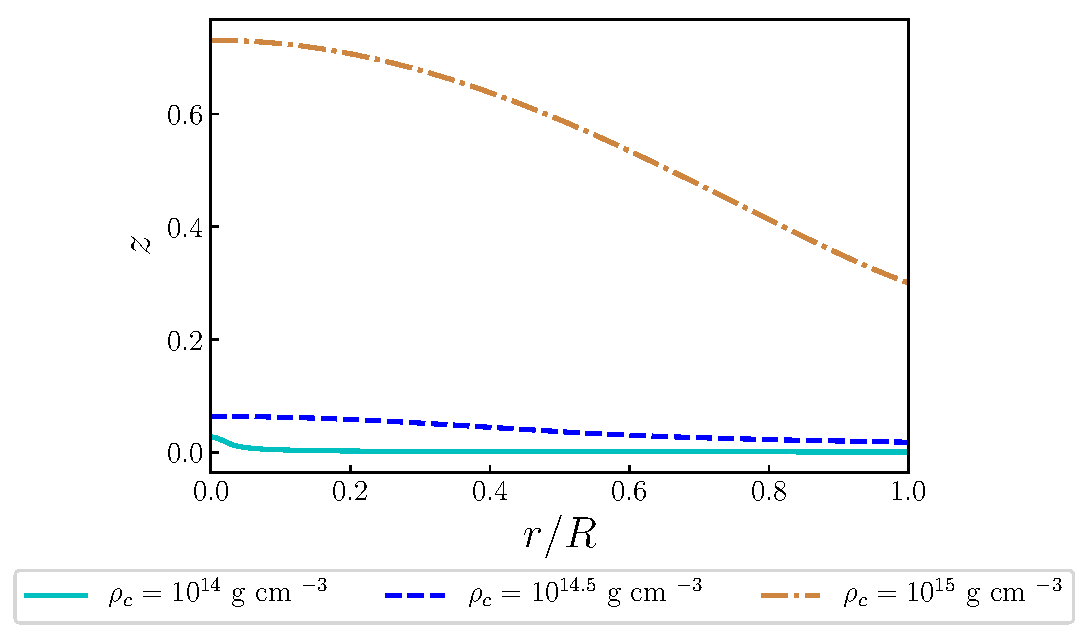
\includegraphics[width=0.93\linewidth]{figures/Redshifteng.pdf}
    \caption{Verificación de C3. Se graficó el corrimiento al rojo $z$ como una función de $r$. Se aprecia que $z$ decrece alcanzando un mínimo en el borde de la estrella para los modelos considerados, satisfaciendo C3.}
    \label{Redshifteng}
\end{figure}

\section{Consolidados}

Tras realizar un análisis análogo al presentado en la sección anterior para todo el conjunto de 37 EOS, los resultados fueron sintetizados en la Tabla \ref{Consolidados}. Se encontró

\begin{table}[H]
\caption{Resultados para las 37 EOSs consideradas. Se listan además el método teórico usado para obtener la EOS, los componentes que interactúan fuertemente (todos los modelos incluyen contribuciones leptónicas), la masa máxima $M_{\text{max}}$ y el respectivo radio $R_{M_{\text{max}}}$ para estrellas estáticas y la referencia a los trabajos originales. }
\label{Consolidados}
\begin{adjustbox}{max width=\textwidth}
\begin{tabular}{ccccccccccc}
\hline
\multirow{2}{*}{\textbf{EOS}} & \multirow{2}{*}{\textbf{Método}}           & \multirow{2}{*}{\textbf{Composición}} & \multirow{2}{*}{\begin{tabular}[c]{@{}c@{}}$\mathbf{M}_{\text{\textbf{max}}}$\\  $[\mathbf{M_{\odot}}]$\end{tabular}} & \multirow{2}{*}{\begin{tabular}[c]{@{}c@{}}$\mathbf{R}_{\mathbf{M}_{\text{\textbf{max}}}}$\\  $[$\textbf{km}$]$\end{tabular}} & \multirow{2}{*}{\textbf{C3}} & \multirow{2}{*}{\textbf{C6}} & \multirow{2}{*}{\textbf{C7}} & \multirow{2}{*}{\textbf{C9}} & \multirow{2}{*}{\textbf{C11}} & \multirow{2}{*}{\textbf{Referencia}}          \\
                     &                                   &                              &                                                                                            &                                                                                           &                     &                     &                     &                     &                      &                                      \\ \hline \addlinespace
ALF1                 & \multirow{4}{*}{Mixto}            & \multirow{4}{*}{$n,p,q$}     & 1.496                                                                                      & 9.221                                                                                     & \checkmark          & \checkmark          & \checkmark          & \checkmark          & \Cross               & \multirow{4}{*}{\cite{Alford2005}}   \\
ALF2                 &                                   &                              & 2.087                                                                                      & 11.962                                                                                    & \checkmark          & \checkmark          & \checkmark          & \checkmark          & \Cross               &                                      \\
ALF3                 &                                   &                              & 1.473                                                                                      & 9.514                                                                                     & \checkmark          & \checkmark          & \checkmark          & \checkmark          & \Cross               &                                      \\
ALF4                 &                                   &                              & 1.943                                                                                      & 10.892                                                                                    & \checkmark          & \checkmark          & \checkmark          & \checkmark          & \Cross               &                                      \\ \addlinespace
AP1                  & \multirow{4}{*}{Variacional}      & \multirow{4}{*}{$n,p$}       & 1.684                                                                                      & 8.292                                                                                     & \checkmark          & \checkmark          & \checkmark          & \checkmark          & \Cross               & \multirow{4}{*}{\cite{Akmal1998}}    \\
AP2                  &                                   &                              & 1.809                                                                                      & 8.746                                                                                     & \checkmark          & \checkmark          & \Cross              & \checkmark          & \Cross               &                                      \\
AP3                  &                                   &                              & 2.391                                                                                      & 10.765                                                                                    & \checkmark          & \Cross              & \Cross              & \checkmark          & \Cross               &                                      \\
AP4                  &                                   &                              & 2.214                                                                                      & 10.004                                                                                    & \checkmark          & \Cross              & \Cross              & \checkmark          & \Cross               &                                      \\ \addlinespace
\end{tabular}
\end{adjustbox}
\end{table}


% Please add the following required packages to your document preamble:
% \usepackage{multirow}
\begin{table}[H]
\renewcommand\thetable{3.1 (continuación)}
\caption{}
\begin{adjustbox}{max width=\textwidth}
\begin{tabular}{ccccccccccc}
\hline
\multirow{2}{*}{\textbf{EOS}} & \multirow{2}{*}{\textbf{Método}}           & \multirow{2}{*}{\textbf{Composición}} & \multirow{2}{*}{\begin{tabular}[c]{@{}c@{}}$\mathbf{M}_{\text{\textbf{max}}}$\\  $[\mathbf{M_{\odot}}]$\end{tabular}} & \multirow{2}{*}{\begin{tabular}[c]{@{}c@{}}$\mathbf{R}_{\mathbf{M}_{\text{\textbf{max}}}}$\\  $[$\textbf{km}$]$\end{tabular}} & \multirow{2}{*}{\textbf{C3}} & \multirow{2}{*}{\textbf{C6}} & \multirow{2}{*}{\textbf{C7}} & \multirow{2}{*}{\textbf{C9}} & \multirow{2}{*}{\textbf{C11}} & \multirow{2}{*}{\textbf{Referencia}}          \\
                     &                                   &                              &                                                                                            &                                                                                           &                     &                     &                     &                     &                      &                                      \\ \hline
ALF1                 & \multirow{4}{*}{Mixto}            & \multirow{4}{*}{$n,p,q$}     & 1.496                                                                                      & 9.221                                                                                     & \checkmark          & \checkmark          & \checkmark          & \checkmark          & \Cross               & \multirow{4}{*}{\cite{Alford2005}}   \\
ALF2                 &                                   &                              & 2.087                                                                                      & 11.962                                                                                    & \checkmark          & \checkmark          & \checkmark          & \checkmark          & \Cross               &                                      \\
ALF3                 &                                   &                              & 1.473                                                                                      & 9.514                                                                                     & \checkmark          & \checkmark          & \checkmark          & \checkmark          & \Cross               &                                      \\
ALF4                 &                                   &                              & 1.943                                                                                      & 10.892                                                                                    & \checkmark          & \checkmark          & \checkmark          & \checkmark          & \Cross               &                                      \\ \addlinespace
AP1                  & \multirow{4}{*}{Variacional}      & \multirow{4}{*}{$n,p$}       & 1.684                                                                                      & 8.292                                                                                     & \checkmark          & \checkmark          & \checkmark          & \checkmark          & \Cross               & \multirow{4}{*}{\cite{Akmal1998}}    \\
AP2                  &                                   &                              & 1.809                                                                                      & 8.746                                                                                     & \checkmark          & \checkmark          & \Cross              & \checkmark          & \Cross               &                                      \\
AP3                  &                                   &                              & 2.391                                                                                      & 10.765                                                                                    & \checkmark          & \Cross              & \Cross              & \checkmark          & \Cross               &                                      \\
AP4                  &                                   &                              & 2.214                                                                                      & 10.004                                                                                    & \checkmark          & \Cross              & \Cross              & \checkmark          & \Cross               &                                      \\ \addlinespace
BBB2                 & Brueckener HF                     & $n,p$                        & 1.920                                                                                      & 9.515                                                                                     & \checkmark          & \checkmark          & \checkmark          & \checkmark          & \Cross               & \cite{Lombardo2004}                  \\ \addlinespace
BGN1H1               & Potencial efectivo                & $n,p,H$                      & 1.630                                                                                      & 9.325                                                                                     & \checkmark          & \checkmark          & \checkmark          & \checkmark          & \Cross               & \cite{Balberg1997}                   \\ \addlinespace
BPAL12               & Brueckener HF                     & $n,p$                        & 1.455                                                                                      & 9.015                                                                                     & \checkmark          & \checkmark          & \checkmark          & \checkmark          & \Cross               & \cite{Zuo1999}                       \\ \addlinespace
BSK19                & \multirow{3}{*}{DFT}              & \multirow{3}{*}{$n,p$}       & 1.861                                                                                      & 9.110                                                                                     & \checkmark          & \Cross              & \Cross              & \checkmark          & \Cross               & \multirow{3}{*}{\cite{Potekhin2013}} \\
BSK20                &                                   &                              & 2.165                                                                                      & 10.173                                                                                    & \checkmark          & \Cross              & \Cross              & \checkmark          & \Cross               &                                      \\
BSK21                &                                   &                              & 2.274                                                                                      & 11.038                                                                                    & \checkmark          & \Cross              & \Cross              & \checkmark          & \Cross               &                                      \\ \addlinespace
ENG                  & Brueckener HF                     & $n,p$                        & 2.241                                                                                      & 10.425                                                                                    & \checkmark          & \checkmark          & \checkmark          & \checkmark          & \Cross               & \cite{Engvik1994}                    \\ \addlinespace
FPS                  & Variacional                       & $n,p$                        & 1.800                                                                                      & 9.279                                                                                     & \checkmark          & \checkmark          & \checkmark          & \checkmark          & \Cross               & \cite{Friedman1981}                  \\ \addlinespace
GNH3                 & Teoría de campos                  & $n,p,H,\Delta$               & 1.965                                                                                      & 11.372                                                                                    & \checkmark          & \checkmark          & \checkmark          & \checkmark          & \Cross               & \cite{Glendenning1985}               \\ \addlinespace
H1                   & \multirow{6}{*}{Teoría de campos} & \multirow{6}{*}{$n,p,H$}     & 1.556                                                                                      & 10.968                                                                                    & \checkmark          & \checkmark          & \checkmark          & \checkmark          & \Cross               & \multirow{6}{*}{\cite{Lackey2006}}   \\
H2                   &                                   &                              & 1.668                                                                                      & 11.516                                                                                    & \checkmark          & \checkmark          & \checkmark          & \checkmark          & \Cross               &                                      \\
H3                   &                                   &                              & 1.790                                                                                      & 11.863                                                                                    & \checkmark          & \checkmark          & \checkmark          & \checkmark          & \Cross               &                                      \\
H4                   &                                   &                              & 2.032                                                                                      & 11.467                                                                                    & \checkmark          & \checkmark          & \checkmark          & \checkmark          & \checkmark           &                                      \\
H5                   &                                   &                              & 1.726                                                                                      & 10.930                                                                                    & \checkmark          & \checkmark          & \checkmark          & \checkmark          & \checkmark           &                                      \\
H7                   &                                   &                              & 1.683                                                                                      & 10.474                                                                                    & \checkmark          & \checkmark          & \checkmark          & \checkmark          & \checkmark           &                                      \\ \addlinespace
MPA1                 & Brueckener HF                     & $n,p$                        & 2.462                                                                                      & 11.301                                                                                    & \checkmark          & \checkmark          & \checkmark          & \checkmark          & \Cross               & \cite{Muther1987}                    \\ \addlinespace
MS1                  & \multirow{2}{*}{Teoría de campos} & \multirow{2}{*}{$n,p$}       & 2.770                                                                                      & 13.346                                                                                    & \checkmark          & \checkmark          & \checkmark          & \checkmark          & \Cross               & \multirow{2}{*}{\cite{Muller1996}}   \\
MS1b                 &                                   &                              & 2.778                                                                                      & 13.301                                                                                    & \checkmark          & \checkmark          & \checkmark          & \checkmark          & \Cross               &                                      \\ \addlinespace
NL3                  & Teoría de campos                  & $n,p,\sigma,\omega,\rho$     & 2.806                                                                                      & 13.427                                                                                    & \checkmark          & \checkmark          & \checkmark          & \checkmark          & \Cross               & \cite{Lalazissis1997}                \\ \addlinespace
PAL6                 & Mixto                             & $n,p$                        & 1.478                                                                                      & 9.258                                                                                     & \checkmark          & \checkmark          & \checkmark          & \checkmark          & \Cross               & \cite{Prakash1988}                   \\ \addlinespace
PCL2                 & Teoría de campos                  & $n,p,H,q$                    & 1.483                                                                                      & 10.116                                                                                    & \checkmark          & \checkmark          & \checkmark          & \checkmark          & \Cross               & \cite{Prakash1995}                   \\ \addlinespace
PS                   & Teoría de campos                  & $n,\pi^0$                    & 1.755                                                                                      & 11.372                                                                                    & \checkmark          & \checkmark          & \checkmark          & \checkmark          & \Cross               & \cite{Pandharipande1975}             \\ \addlinespace
SLy                  & Mixto                             & $n,p$                        & 2.050                                                                                      & 9.977                                                                                     & \checkmark          & \checkmark          & \Cross              & \checkmark          & \Cross               & \cite{Douchin2001}                   \\ \addlinespace
SQM1                 & \multirow{3}{*}{Teoría de campos} & \multirow{3}{*}{$q$}         & 1.532                                                                                      & 8.315                                                                                     & \checkmark          & \checkmark          & \checkmark          & \checkmark          & -                    & \multirow{3}{*}{\cite{Prakash1995}}  \\
SQM2                 &                                   &                              & 1.737                                                                                      & 9.638                                                                                     & \checkmark          & \checkmark          & \checkmark          & \checkmark          & -                    &                                      \\
SQM3                 &                                   &                              & 1.977                                                                                      & 10.814                                                                                    & \checkmark          & \checkmark          & \checkmark          & \checkmark          & -                    &                                      \\ \addlinespace
WFF1                 & \multirow{3}{*}{Variacional}      & \multirow{3}{*}{$n,p$}       & 2.134                                                                                      & 9.413                                                                                     & \checkmark          & \checkmark          & \Cross              & \checkmark          & \Cross               & \multirow{3}{*}{\cite{Wiringa1988}}  \\
WFF2                 &                                   &                              & 2.199                                                                                      & 9.825                                                                                     & \checkmark          & \checkmark          & \Cross              & \checkmark          & \Cross               &                                      \\
WFF3                 &                                   &                              & 1.845                                                                                      & 9.516                                                                                     & \checkmark          & \checkmark          & \checkmark          & \checkmark          & \Cross               &                                      \\ \addlinespace
\end{tabular}
\end{adjustbox}
\end{table}